\documentclass[a4paper]{article}%字号5号
\usepackage{xpatch}
\ExplSyntaxOn
\makeatletter
\xpatchcmd{\@maketitle}
{
    \@title
}
{
    \heiti\zihao{3}\@title
}
{}{\fail}
\xpatchcmd{\@maketitle}
{
    \@author
}
{
    \kaishu\zihao{-4}\@author
}
{}{\fail}
\makeatother
\ExplSyntaxOff
\usepackage{ctex}%输出汉字
\usepackage{times}%英文字体
\title{对于迭代数列$x_{n+1}=x_n^2/2+c/2,x_1=c/2$行为的探究}%黑体三号,行距1.5倍
\author{范潇\phantom{1}陈思同\phantom{1}吴靖阳}%小四字号,1.5倍行距,仿宋
\date{}%去除日期
\linespread{1.5}%行间距1.5倍
\usepackage{amsmath,amsthm,amssymb,graphicx}
\usepackage[]{pifont}
\usepackage{float}
\usepackage{caption}
\usepackage{unicode-math}
\usepackage{setspace}
\usepackage{subfigure}
\usepackage[export]{adjustbox}%防止过宽的图片
\usepackage{bibentry,natbib}%两个参考文献宏包
\usepackage{abstract}
\usepackage{fontspec}
\usepackage{xeCJK}
\setCJKmainfont{SimSun}
\setCJKsansfont{SimSun}
\setCJKmonofont{SimSun}%正文字体为宋体
\usepackage[fontsize=10.5pt]{fontsize}
\renewcommand{\abstracttextfont}{\fangsong}%摘要字体改为仿宋
\renewcommand{\abstractname}{\textbf{摘\quad 要}}%更改摘要两字的样式
\usepackage{indentfirst}%中文首行缩进
\usepackage[left=2.50cm,right=2.50cm,top=2.80cm,bottom=2.50cm]{geometry}%页边距设置
\bibliographystyle{unsrt}%让引用序号按照顺序排列
\newtheorem{thm}{定理}
\newtheorem{definiton}{定义}
\newcommand*\abs[1]{\lvert#1\rvert}%绝对值符号
\newcommand\Emph{\textbf}%粗体强调命令
\usepackage{indentfirst}
\begin{document}
  \maketitle  
\begin{abstract}
迭代数列$x_{n+1}=\frac{1}{2}x_{n}^2+\frac{1}{2}c,x_1=\frac{1}{2}c$是一个一维二次映射.
函数$f(x)=\frac{1}{2}x^2+\frac{1}{2}c$是一个$\mathbb{R} \to \mathbb{R} $,光滑且连续的函数.
在这样的一个系统中,很多初始值在经过多次迭代后,往往会稳定在某些状态中.
这些状态不一定是稳定在某个不动点,而有可能是持续运动的——$x_n$可能会在实数轴上不断“跳跃”.
而这则会导致当控制参数c到达一定大小后该迭代数列会产生混沌现象.\\
\end{abstract}

\section{一些定义和定理}

\begin{definiton}不动点 \phantom{1}
    设函数$F(x)$在区间$I$上有定义,若存在$x^*\in I$满足$F(x^*)=x^*$,则称$x^*$为$F(x)$在$I$上的不动点.\end{definiton}
\begin{thm}当$\abs{dF(x)/dx}_{x^*}<1$我们称$x^*$为一个稳定的不动点,当$x_1$在$x^*$附近时,$x_n$最终会收敛于该稳定点$x^*$.\cite{e}\end{thm}
\begin{definiton}周期点 \phantom{1}\\记\[F^{0}(x)=x,F^{n+1}(x)=F(F^{n}(x))\]
如果
$F^{n}(x^*)=x^*$且$F^{k}(x^*)\neq x^*$\phantom{1}$(k<n)$,
则称$x^*$为n周期点$(n=0,1,2,\cdots )$ .如果m是某个正整数且$p=F^{m}(q)$是周期点,则我们称q是为最终周期点.\end{definiton}

\begin{definiton}Schwarzian导数 \phantom{1}
函数$F(x)$的Schwarzian导数被定义为\[\{F,x\}\equiv \frac{F^{\prime \prime \prime }}{F^{\prime}}-\frac{3}{2}(\frac{F^{\prime \prime}}{F^{\prime}})^2.\]
\end{definiton}
\section{迭代数列的大致行为}

\subsection{$c\in (-\infty ,-8)\cup  (1,\infty)$时的行为}
当$c>1$时,\[x_{n+1}-x_{n}=\frac{1}{2}x_n^2+\frac{1}{2}c-x_n=\frac{1}{2}(x_n-1)^2+\frac{1}{2}(c-1)\ge\frac{1}{2}(c-1)>0,\]
易知数列$\{x_n\}$发散至正无穷.

当$c<-8$时,\[x_2=\frac{1}{2}x_1^2+\frac{1}{2}c=\frac{(c+2)^2-4}{8}>4>\frac{1}{2},\]
因此$c<-8$的情况可以视为$c>1$时的情况,即数列$\{x_n\}$发散至正无穷.

综上,当$c\in (-\infty ,-8)\cup  (1,\infty)$时,数列$\{x_n\}$发散至正无穷.
\subsection{$c=-8$时的行为}
由迭代关系可知,\[x_1=-4,x_2=x_3=\ldots =x_n=4\phantom{1}(n\ge2),\]
即数列$\{x_n\}$收敛于4.
\subsection{$c=1$时的行为}
此时\[x_{n+1}-x_n=\frac{1}{2}(x_n-1)^2\ge0,\]
因此数列$\{x_n\}$单调递增.由数学归纳法易证1为数列$\{x_n\}$的一个上界.由单调有界定理可知,数列$\{x_n\}$存在极限.对等式\[x_{n+1}=\frac{1}{2}x_{n}^2+\frac{1}{2}c,\]等号两边同时取极限后可得\[\lim _{x\to\infty}{x_n}=1,\]
即数列$\{x_n\}$收敛于1.
\subsection{$c\in (-8,1)$时的行为}
%插入图一(该图片的标题为"$c\in(-8,1)$时的分岔图")
\begin{figure}[H]
    \centering
    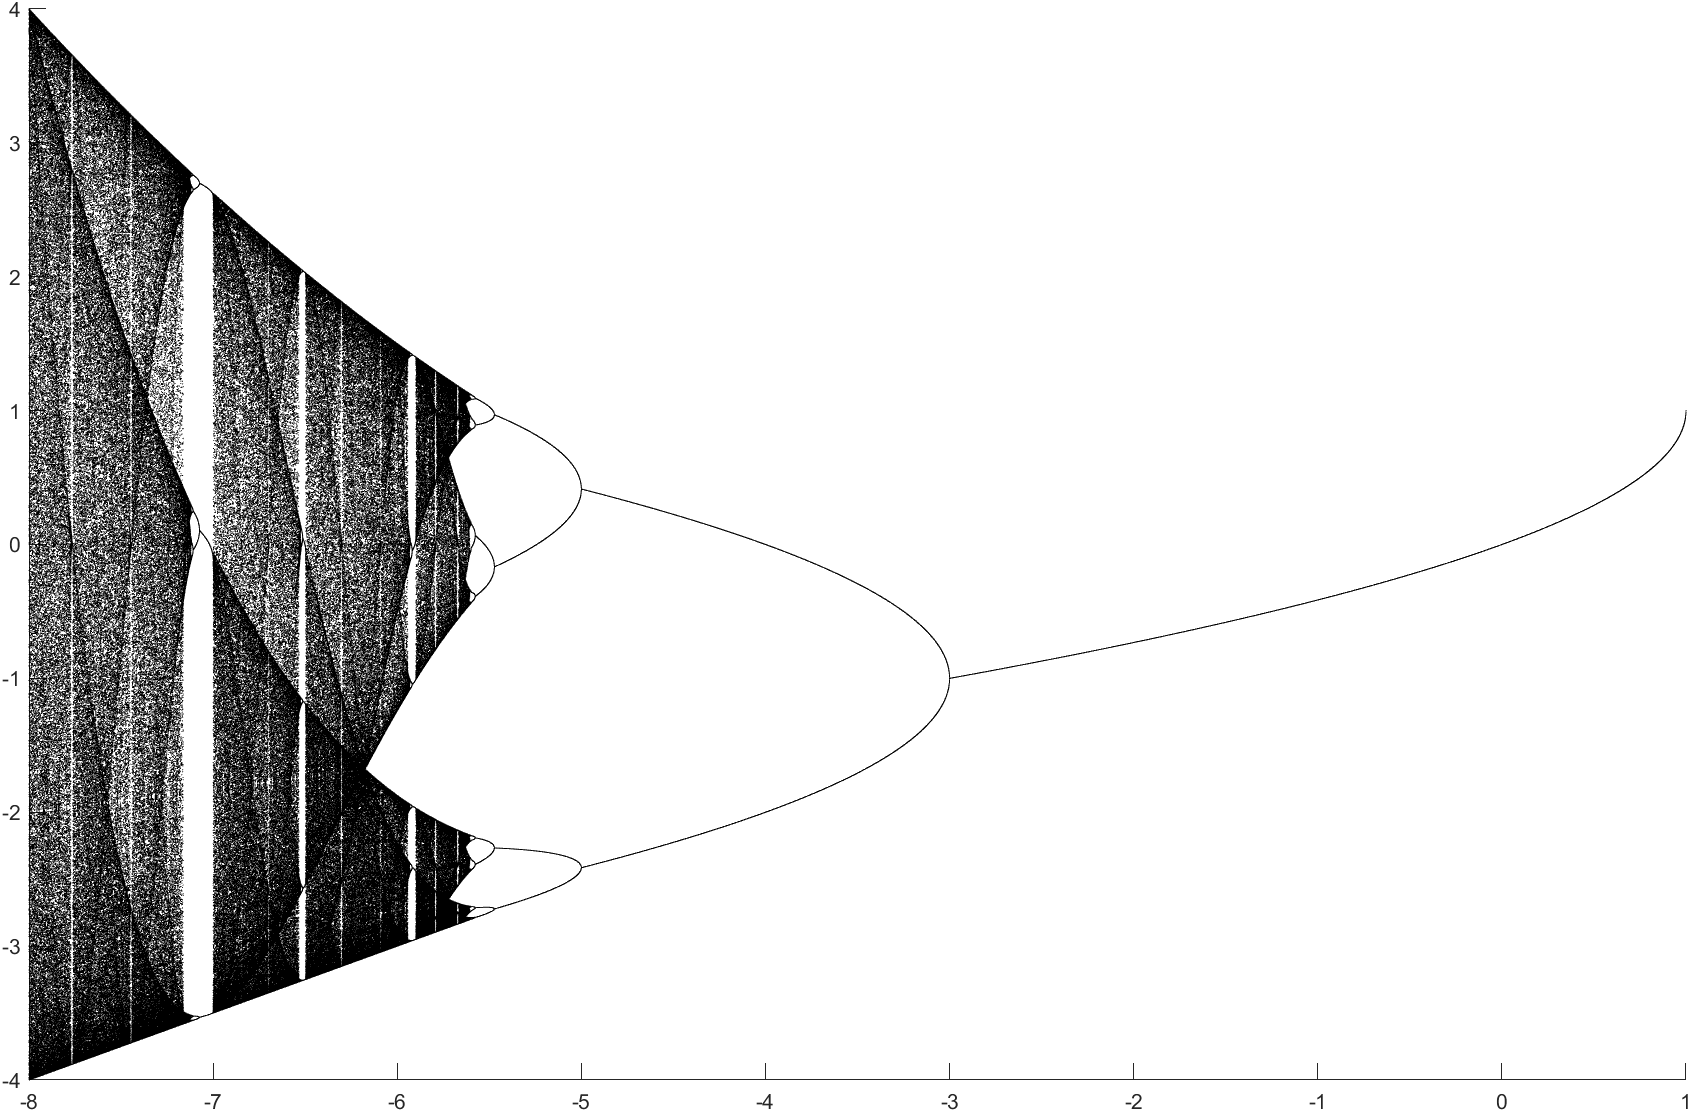
\includegraphics[scale=0.3]{图一}
    \caption[图一]{$c\in(-8,1)$时的分岔图}\label{fig-图一}
    \end{figure}
{\zihao{-5}\CJKfamily{zhkai}本张图绘制了90000个c值,间隔0.0001.对于每个c值都预先迭代5000000次,再将之后的25次迭代结果绘制在图中.}

当$c\in (-3,1)$时
由方程$f(x^*)=x^*$可解得不动点为$x^{*}=1-\sqrt{1-c}$\\
因
\[ \abs{df(x)/dx}_{x^*}<1,\]由{\zihao{5}\CJKfamily{zhhei}定理1}可知该不动点稳定.如所示图2,$x_n$最终会收敛于该点.
%插入图二(该图片的标题为"c=-2")
\begin{figure}[ht]
    \centering
    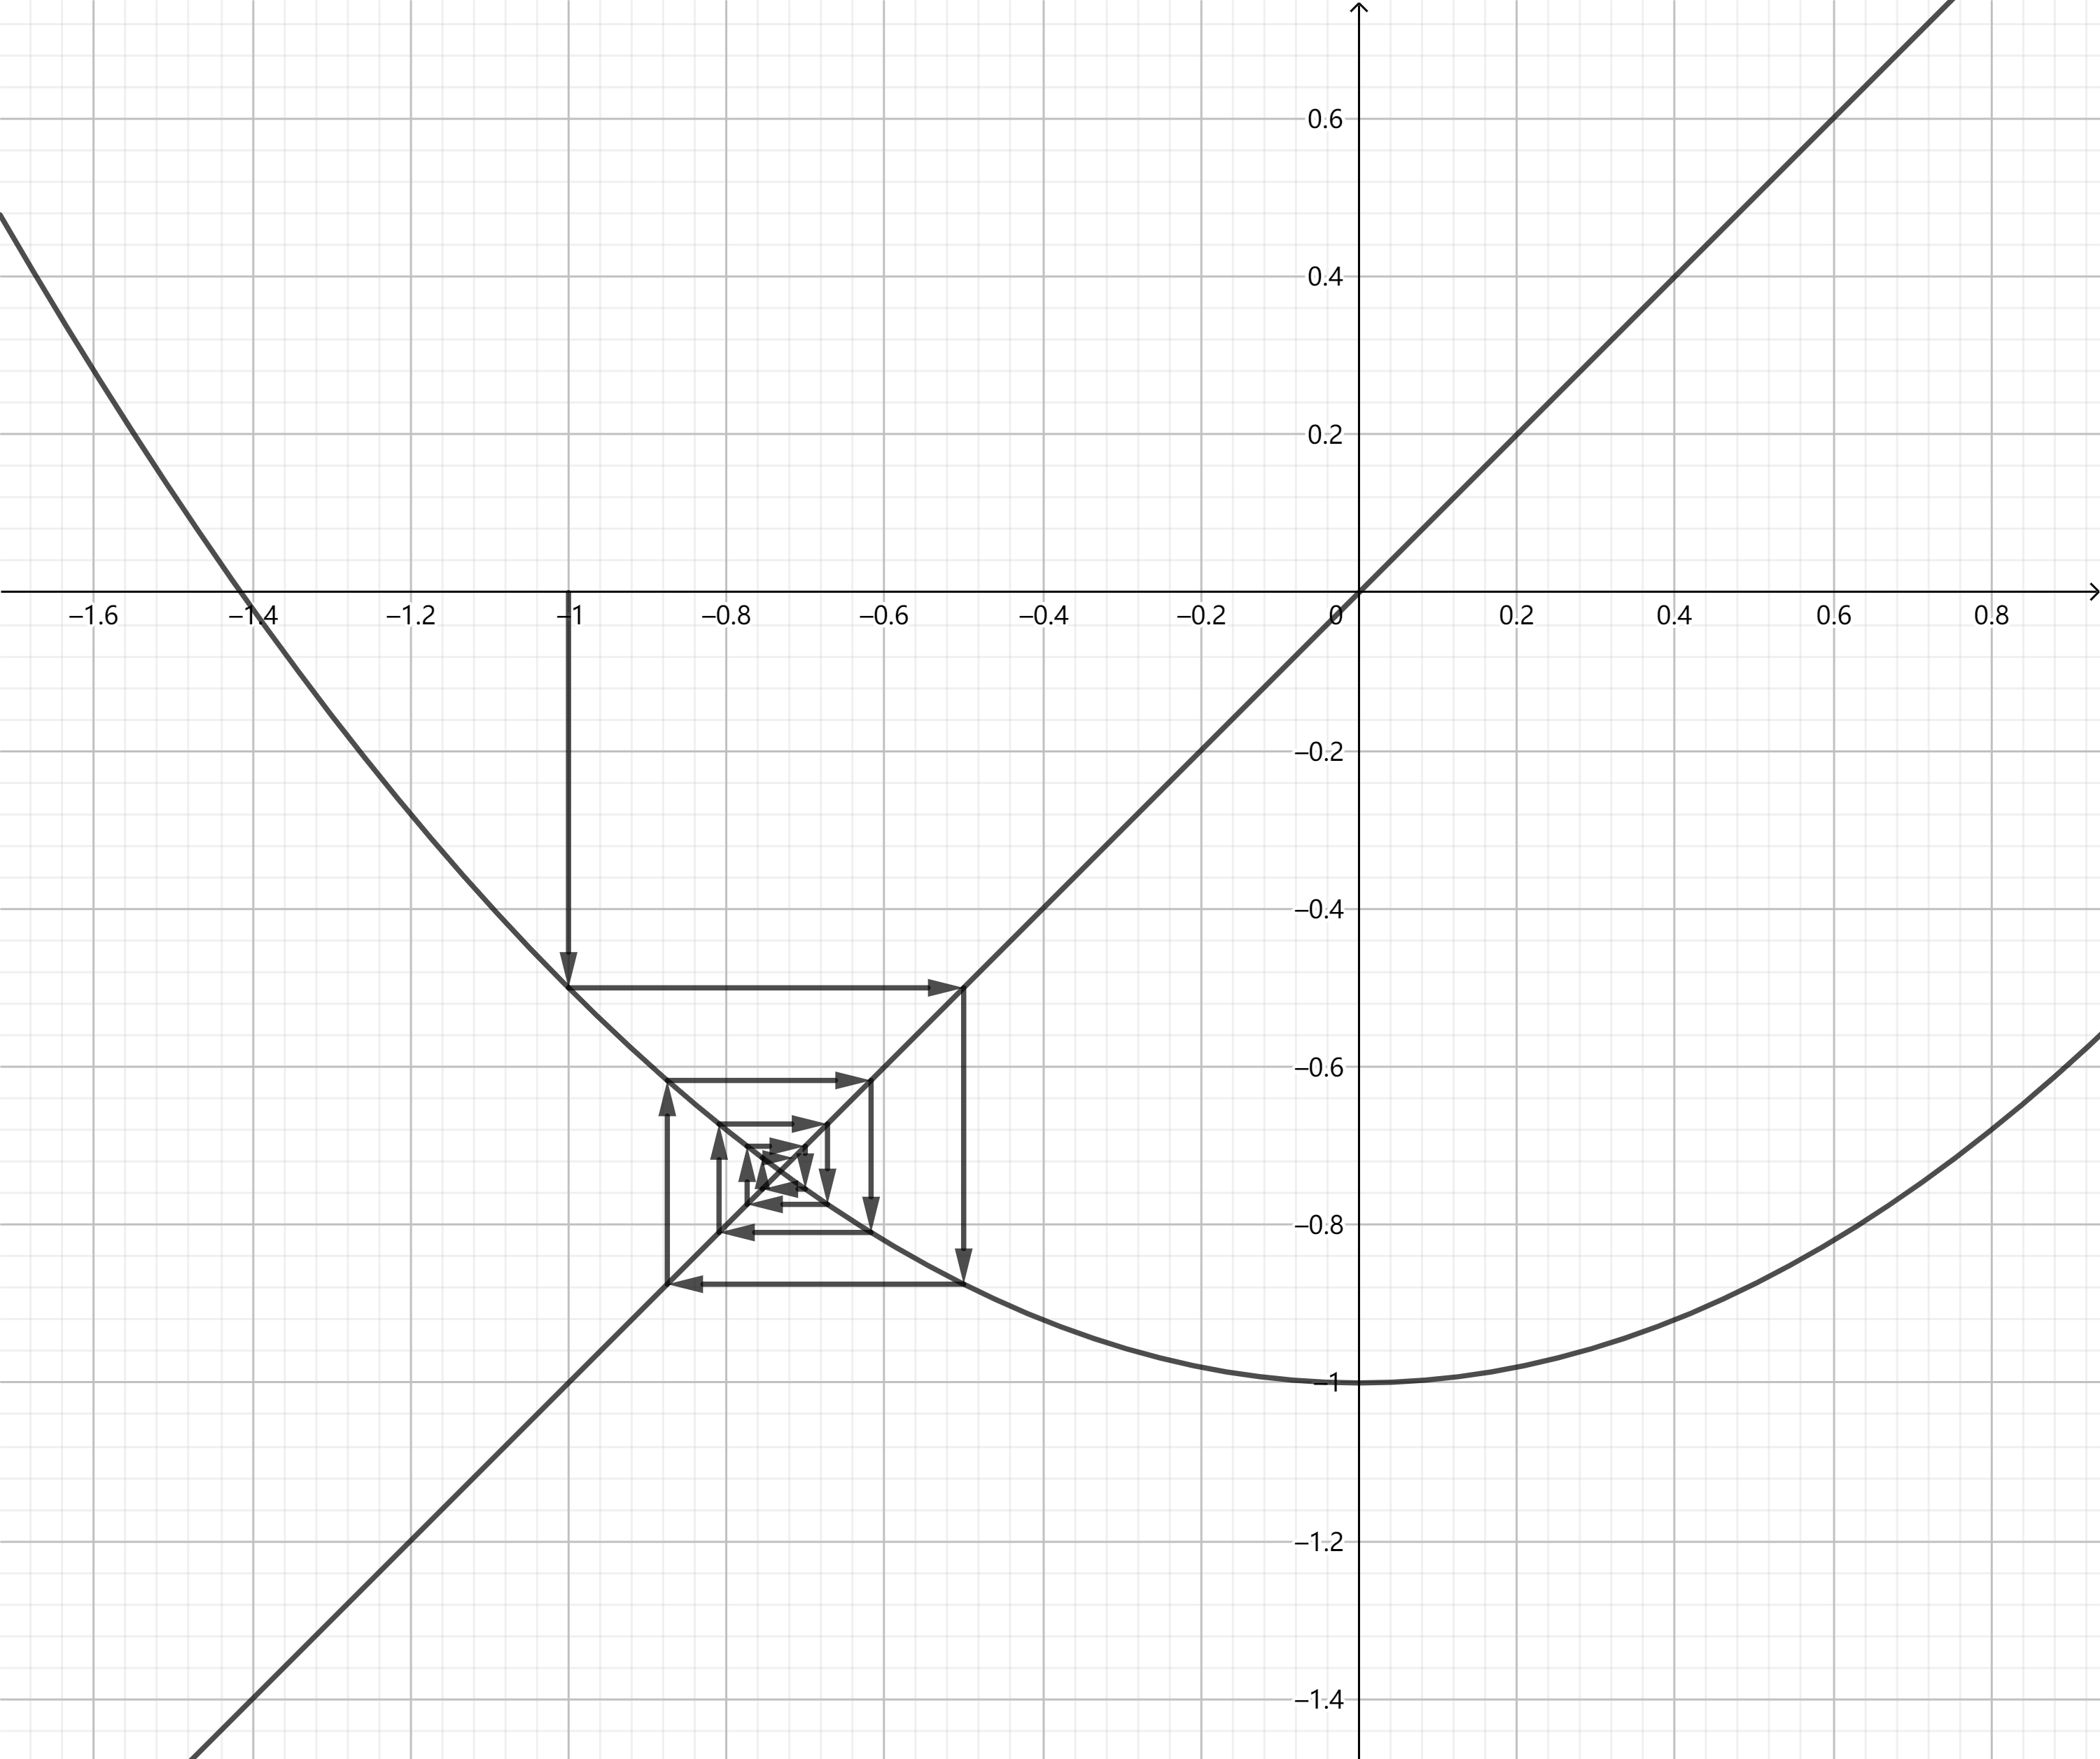
\includegraphics[scale=4.8]{图二}
    \caption[图二]{$c=-2$}\label{fig-图二}
    \end{figure}


当控制参数c不断减小直至小于-3后,
\[\abs{df(x)/dx}_{x^*}\ge1,\]
该不动点变得不稳定.$x_n$经过多次迭代后最终会在$x^*_1$和$x^*_2$两点间不断摆动.\\
即
\[f(x^*_1)=x^*_2,f(x^*_2)=x^*_1,\]
也就是说这两点迭代两次后会得到原先的值,\\
即
\[f^{2}(x^*_k)=f(f(x^*_k))=x^*_k \phantom{1} (k=1,2),\]
\begin{figure}[h]
    \centering
    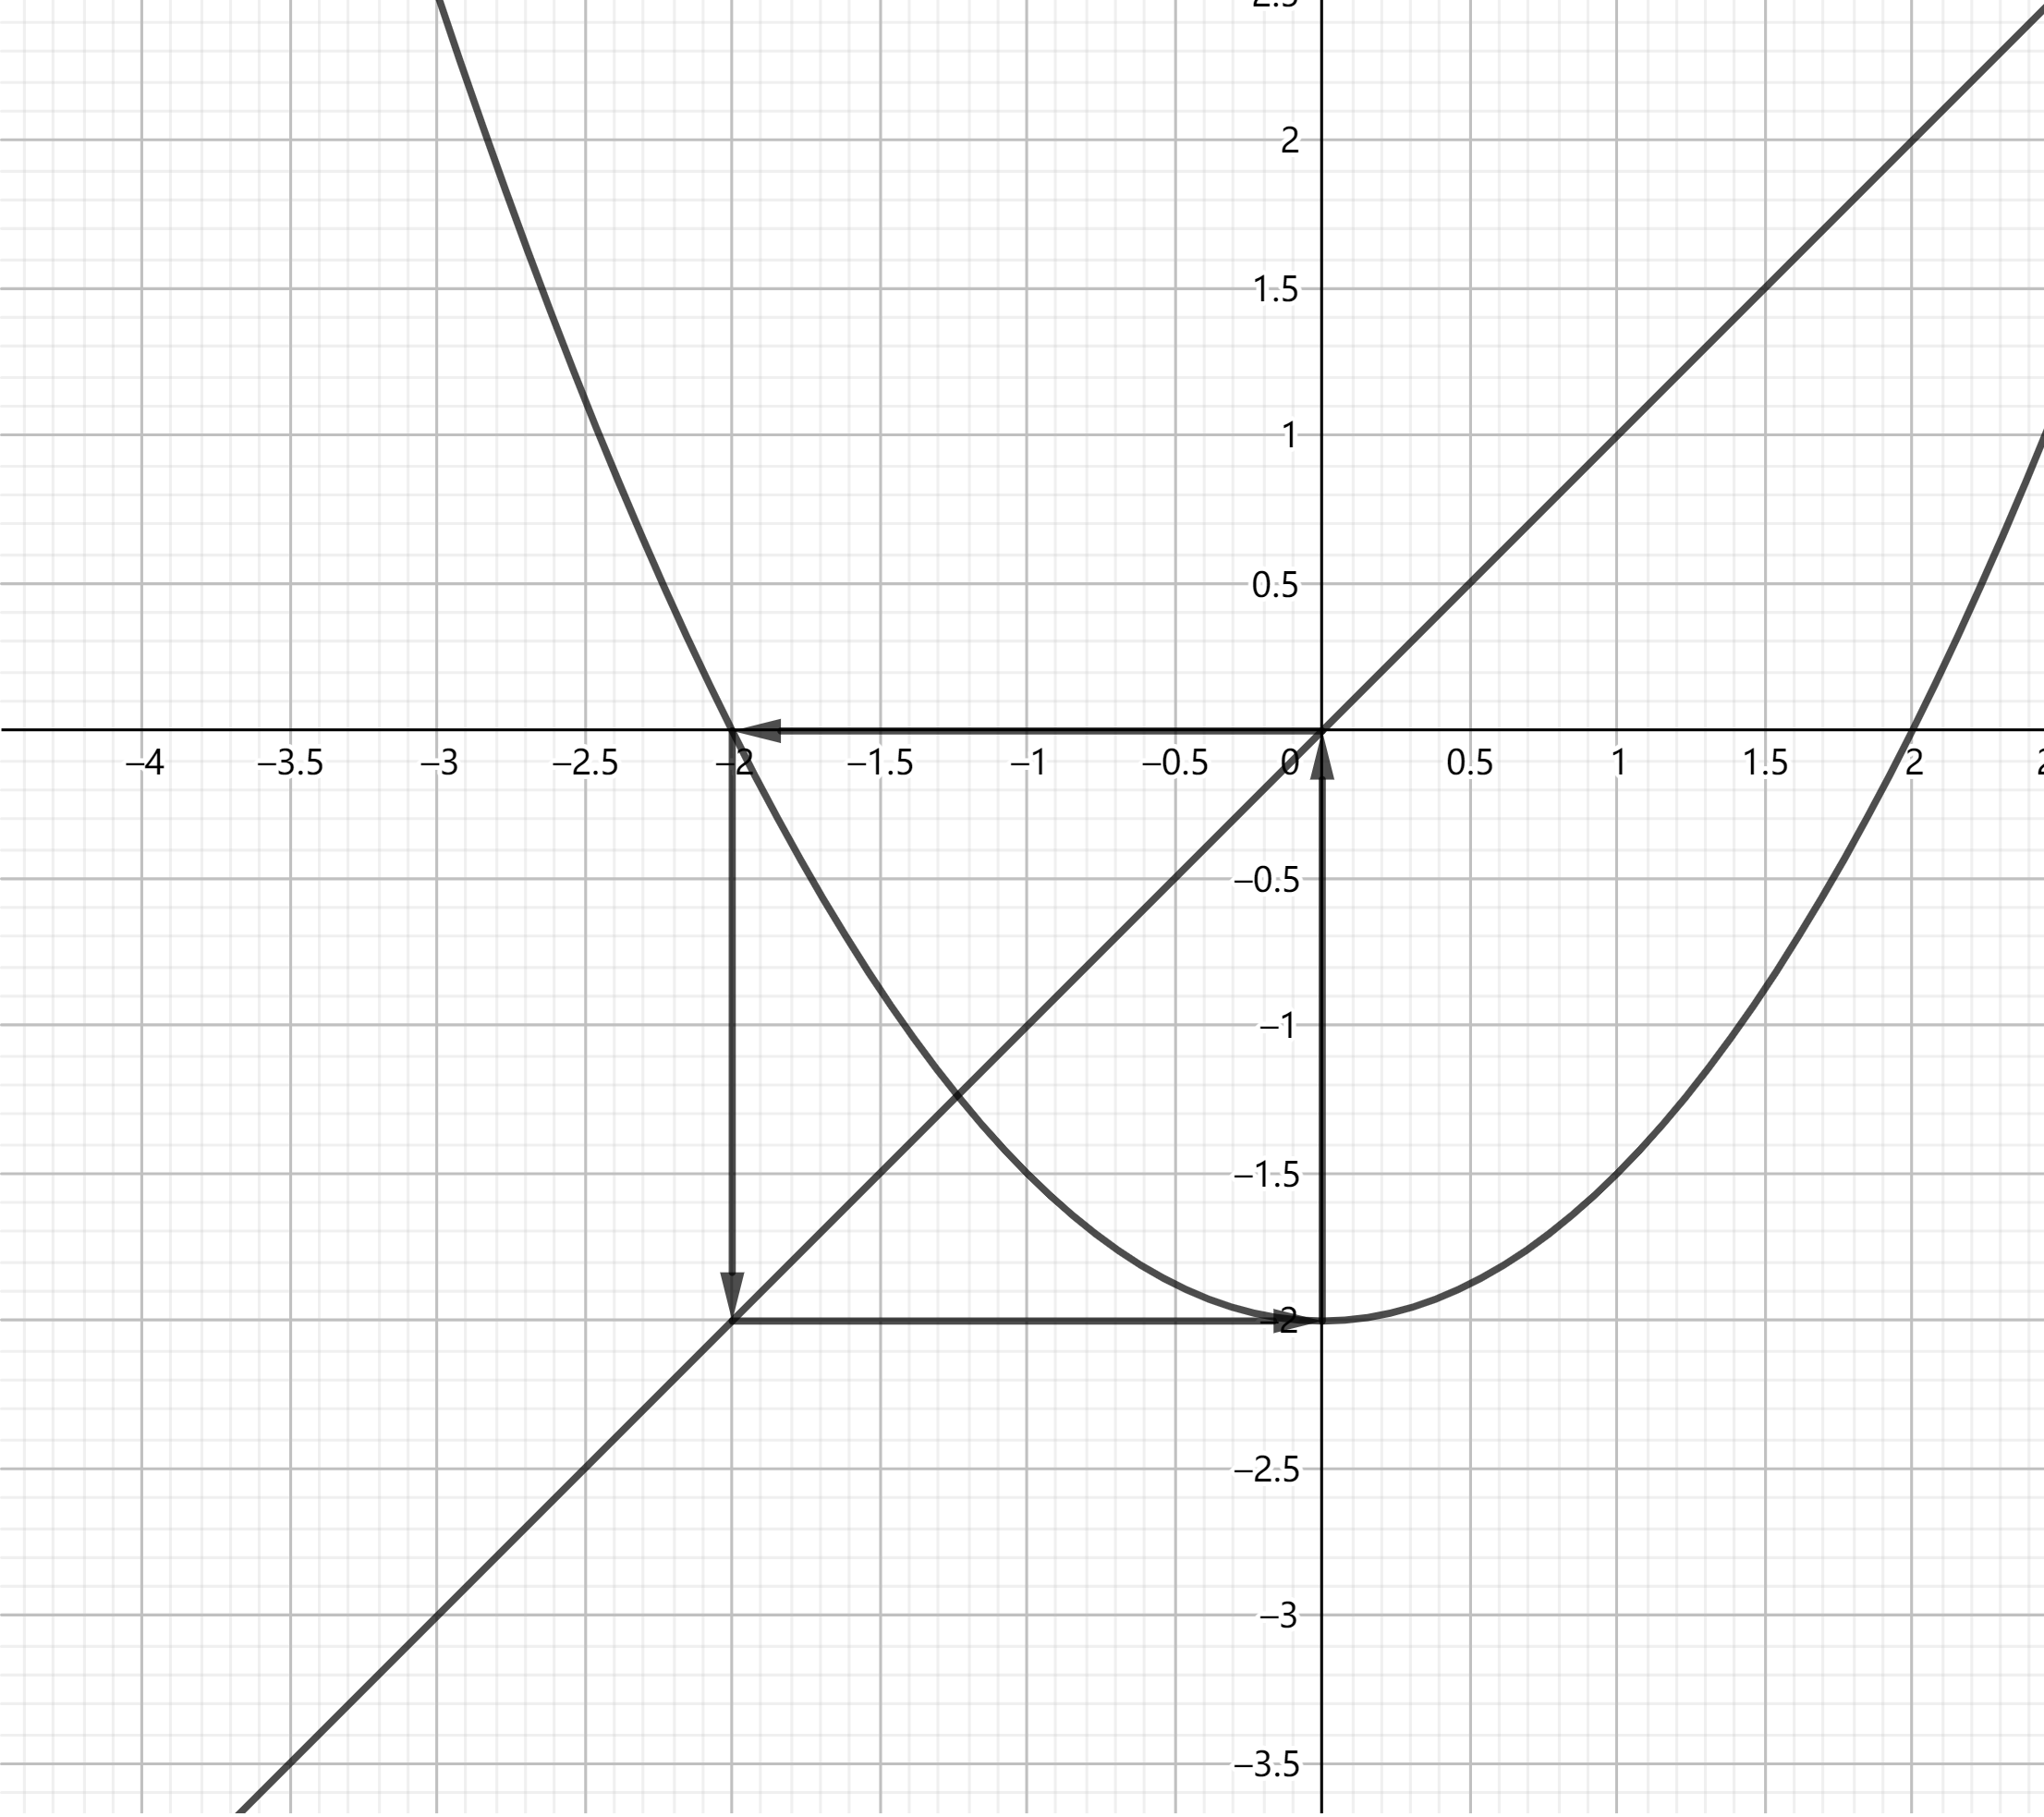
\includegraphics[scale=1.8]{图三}
    \caption[图三]{$c=-4$}\label{fig-图三}
    \end{figure}
这两个点便是$f^2(x)$的不动点.
此时这两个不动点都是稳定的.
%插入图三(该图片的标题为"c=-4")

控制参数c减小并越过-3前后发生的迭代数列行为上的变化导致了图1中在$c=-3$处出现了开口向左的叉形分岔.
我们记$c_1=-3$.
当控制参数c继续减小,这两个不动点将变得不稳定,我们记临界点为$c_2$.在分岔图中,在该点处产生了两处分岔,使迭代数列产生了$2^2=4$周期循环.
随着控制参数c继续减小,上述的4周期循环又将不稳定,产生8周期循环.这样的周期不断加倍的过程将不断重复,表现为分岔图上从右往左,一分二,二分四,四分八,八分十六……不断持续下去的叉形分岔.
有以下结论:
如果$c_{n+1}\le c<c_n$,那么迭代数列会有稳定的$2^n$周期循环
同时
$\lim_{x\to\infty}c_n\equiv c_{\infty}$(有限值)
通过计算可以得到如下数据:\\
%插入表一
\begin{center}
\begin{tabular}{|c|r@{.}l|}
    \hline
$c_{1}$ & -3&0000 \\ \hline
$c_{2}$ & -5&0000 \\ \hline
 $c_{3}$ & -5&5761 \\ \hline
 $c_{4}$ & -5&5985 \\ \hline
 $c_{5}$ & -5&6033 \\ \hline
 $c_{6}$ & -5&6043 \\ \hline
 $c_{\infty}$ & -5&6051 \\ \hline
\end{tabular}
\end{center}

有\[\delta =\lim_{n\to\infty}\frac{c_{n+1}-c_n}{c_{n+2}-c_{n+1}}\]
为一个常数\cite{a}.
称为\textsl{Feigenbaum}常数.
对于所有\textsl{Schwarzian}导数为负数的一维映射,\textsl{Feigenbaum}常数均为$\delta=4.669201609102990$.\cite{b}
因此$x_{n+1}=\frac{1}{2}x_{n}^2+\frac{1}{2}c$的\textsl{Feigenbaum}常数为$\delta=4.669201609102990$.

当$c<c_{\infty}$时,迭代数列$x_{n+1}=\frac{1}{2}x_{n}^2+\frac{1}{2}c$
不仅会产生无穷多个不稳定的$2^n$周期解,也会产生新的稳定周期解(如$3*x^n,5*x^n$等),同时还会产生非周期性的解.这些情况都由控制参数c来决定.

其中非周期的解的含义是一个点被周期性的在$2^n$个不相交的实数轴上的范围之间不断映射,却不是周期点(或最终周期点).这种非周期性的数列被称为“半周期”数列\cite{c}
当c小于$c_{\infty}$时,这些在实数轴上不相交的范围的数量随着c增大而趋向无穷,也就是说,在实数轴上不相交的范围的数量会随着c减小而较小,这在分岔图上呈现为开口朝右的逆分岔.
%插入图四,标题为:形如"<"的逆分岔
\begin{figure}[ht]
    \centering
    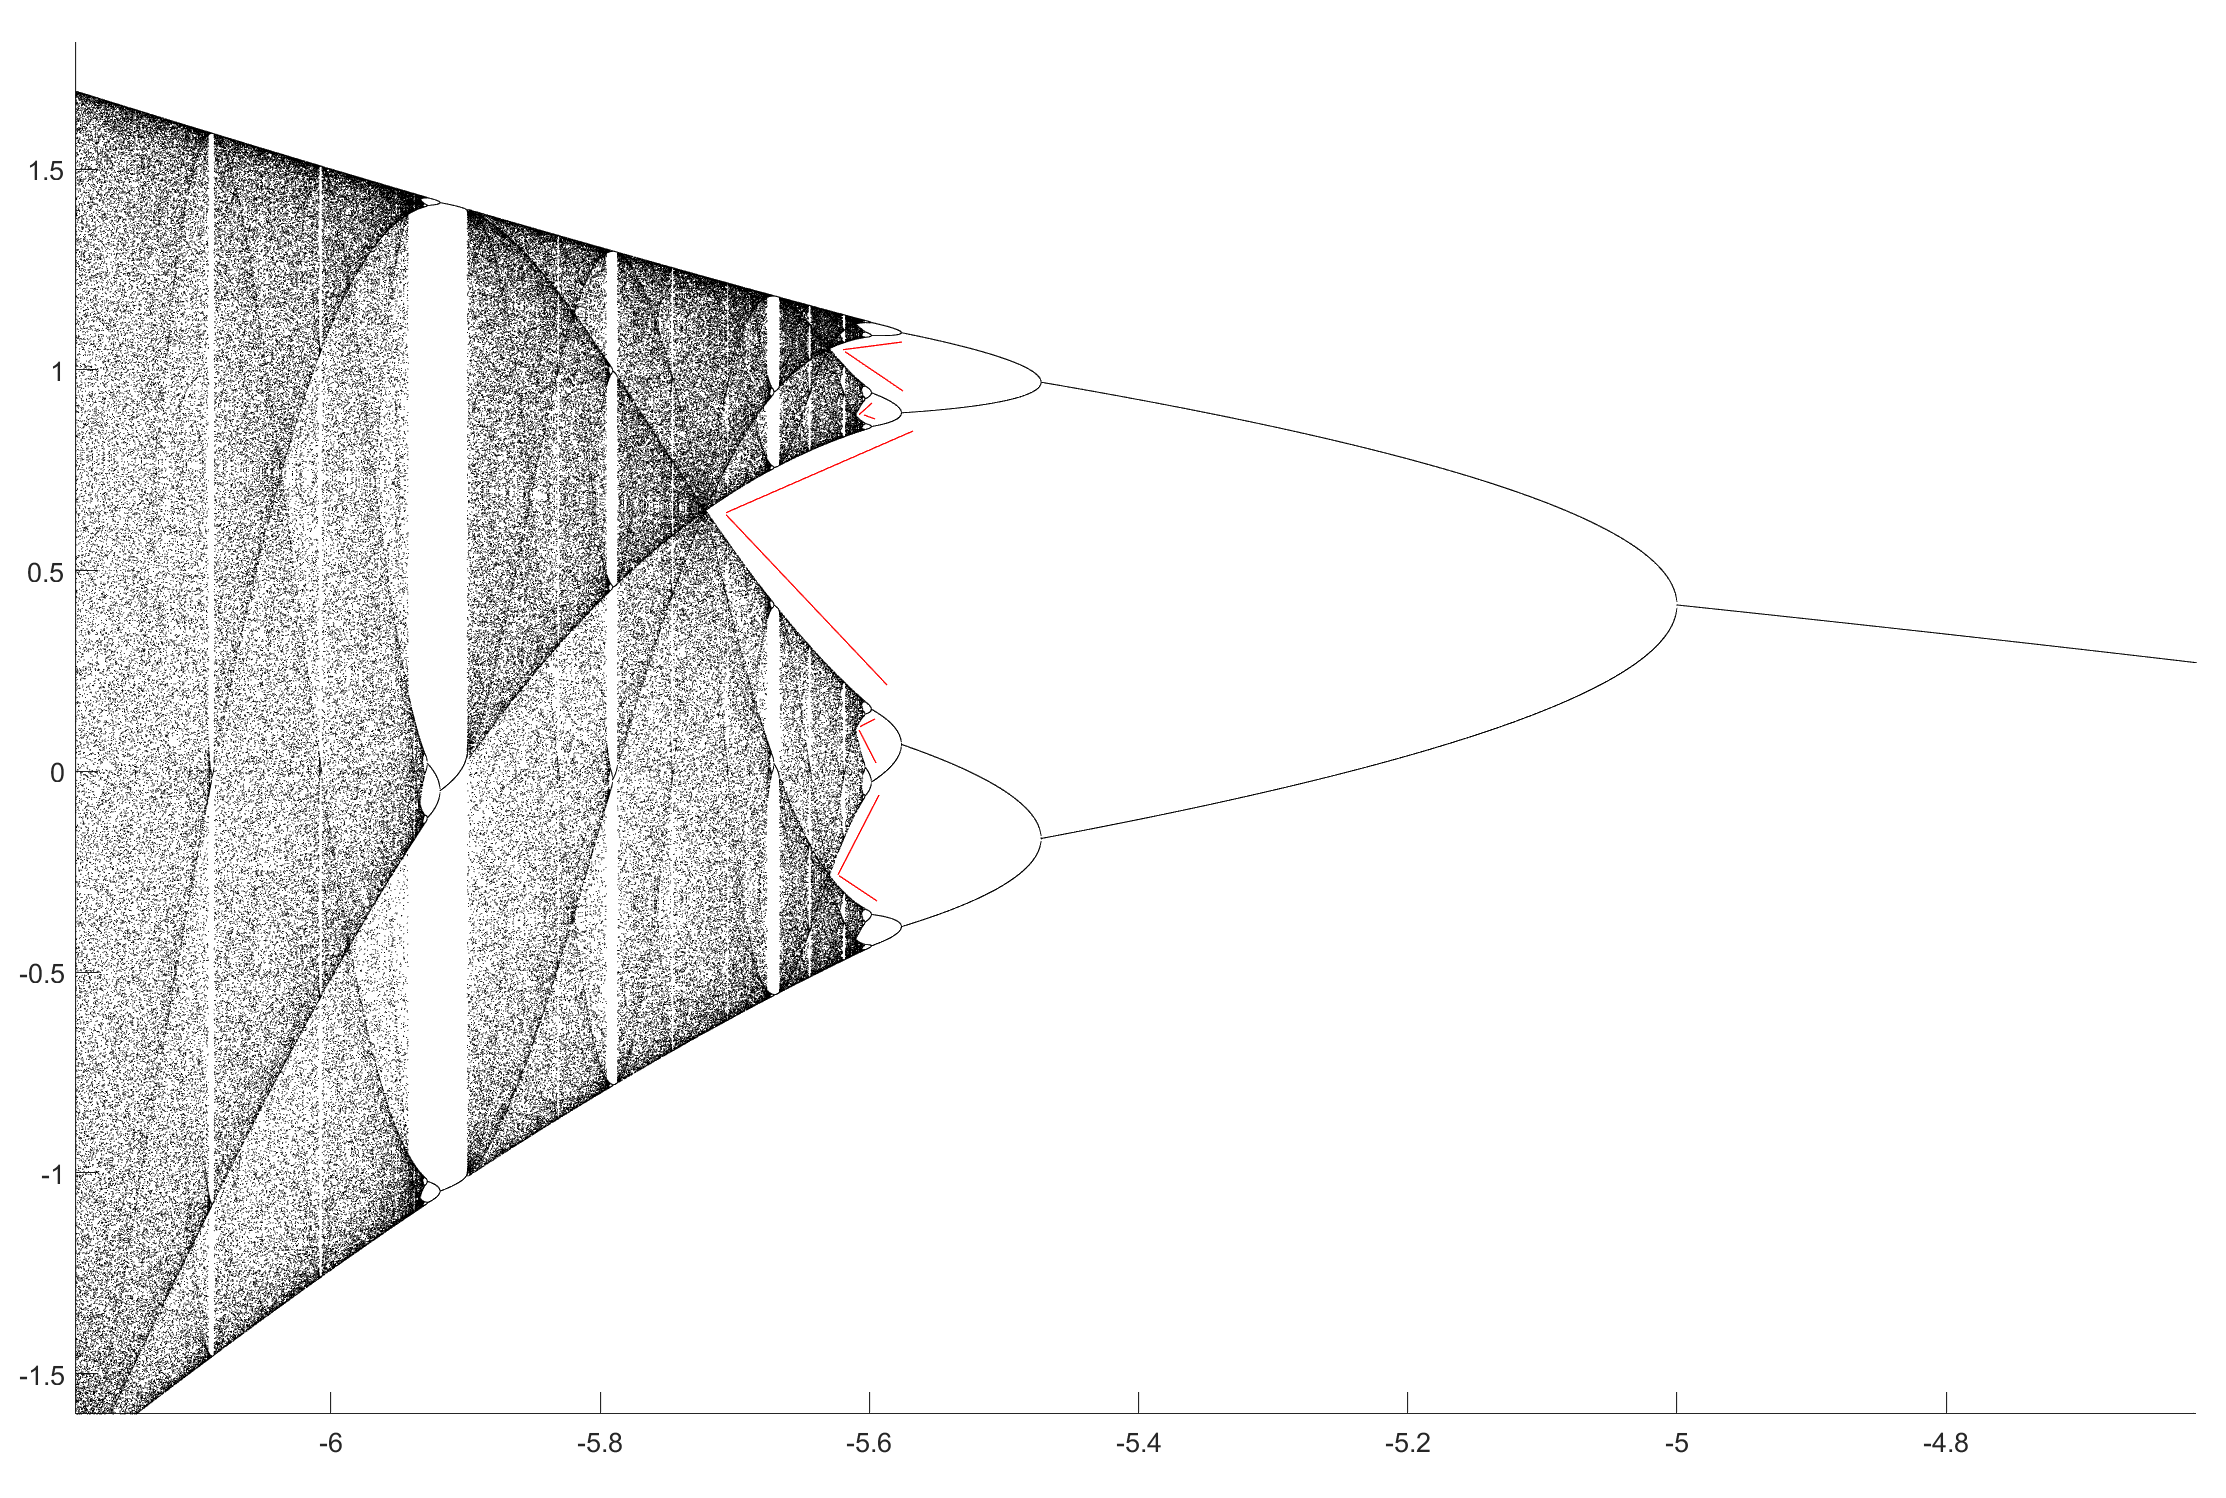
\includegraphics[scale=0.27]{图四}
    \caption[图四]{形如"<"的逆分岔}\label{fig-图四}
    \end{figure}


从分岔图中可知,这些范围随着c减小而拓宽,然后重叠.


当$c=-6.1746\ldots $时,这些范围连接在一起,当c小于这个值时,即使$x_n$周期性地在这些范围内,但是以一种飘忽不定的方式在这些范围内跳跃,尽管是确定的,但是对于初始值的变化十分敏感.这种状态称为混沌.\cite{c}

\section{相切分岔现象}

当c=-7时,$F^{3}(x)$与$y=x$于它的三个极值点相切,
%插入图五,无标题

而这会导致迭代数列$x_{n+1}=\frac{1}{2}x_{n}^2+\frac{1}{2}c$产生稳定的3周期循环,称为相切分岔现象.
而这也会导致“间歇现象”,在分岔图中体现为$c=-7$左侧类似于收起的帷幕的形状\cite{c}
\begin{figure}[ht]
    \centering
    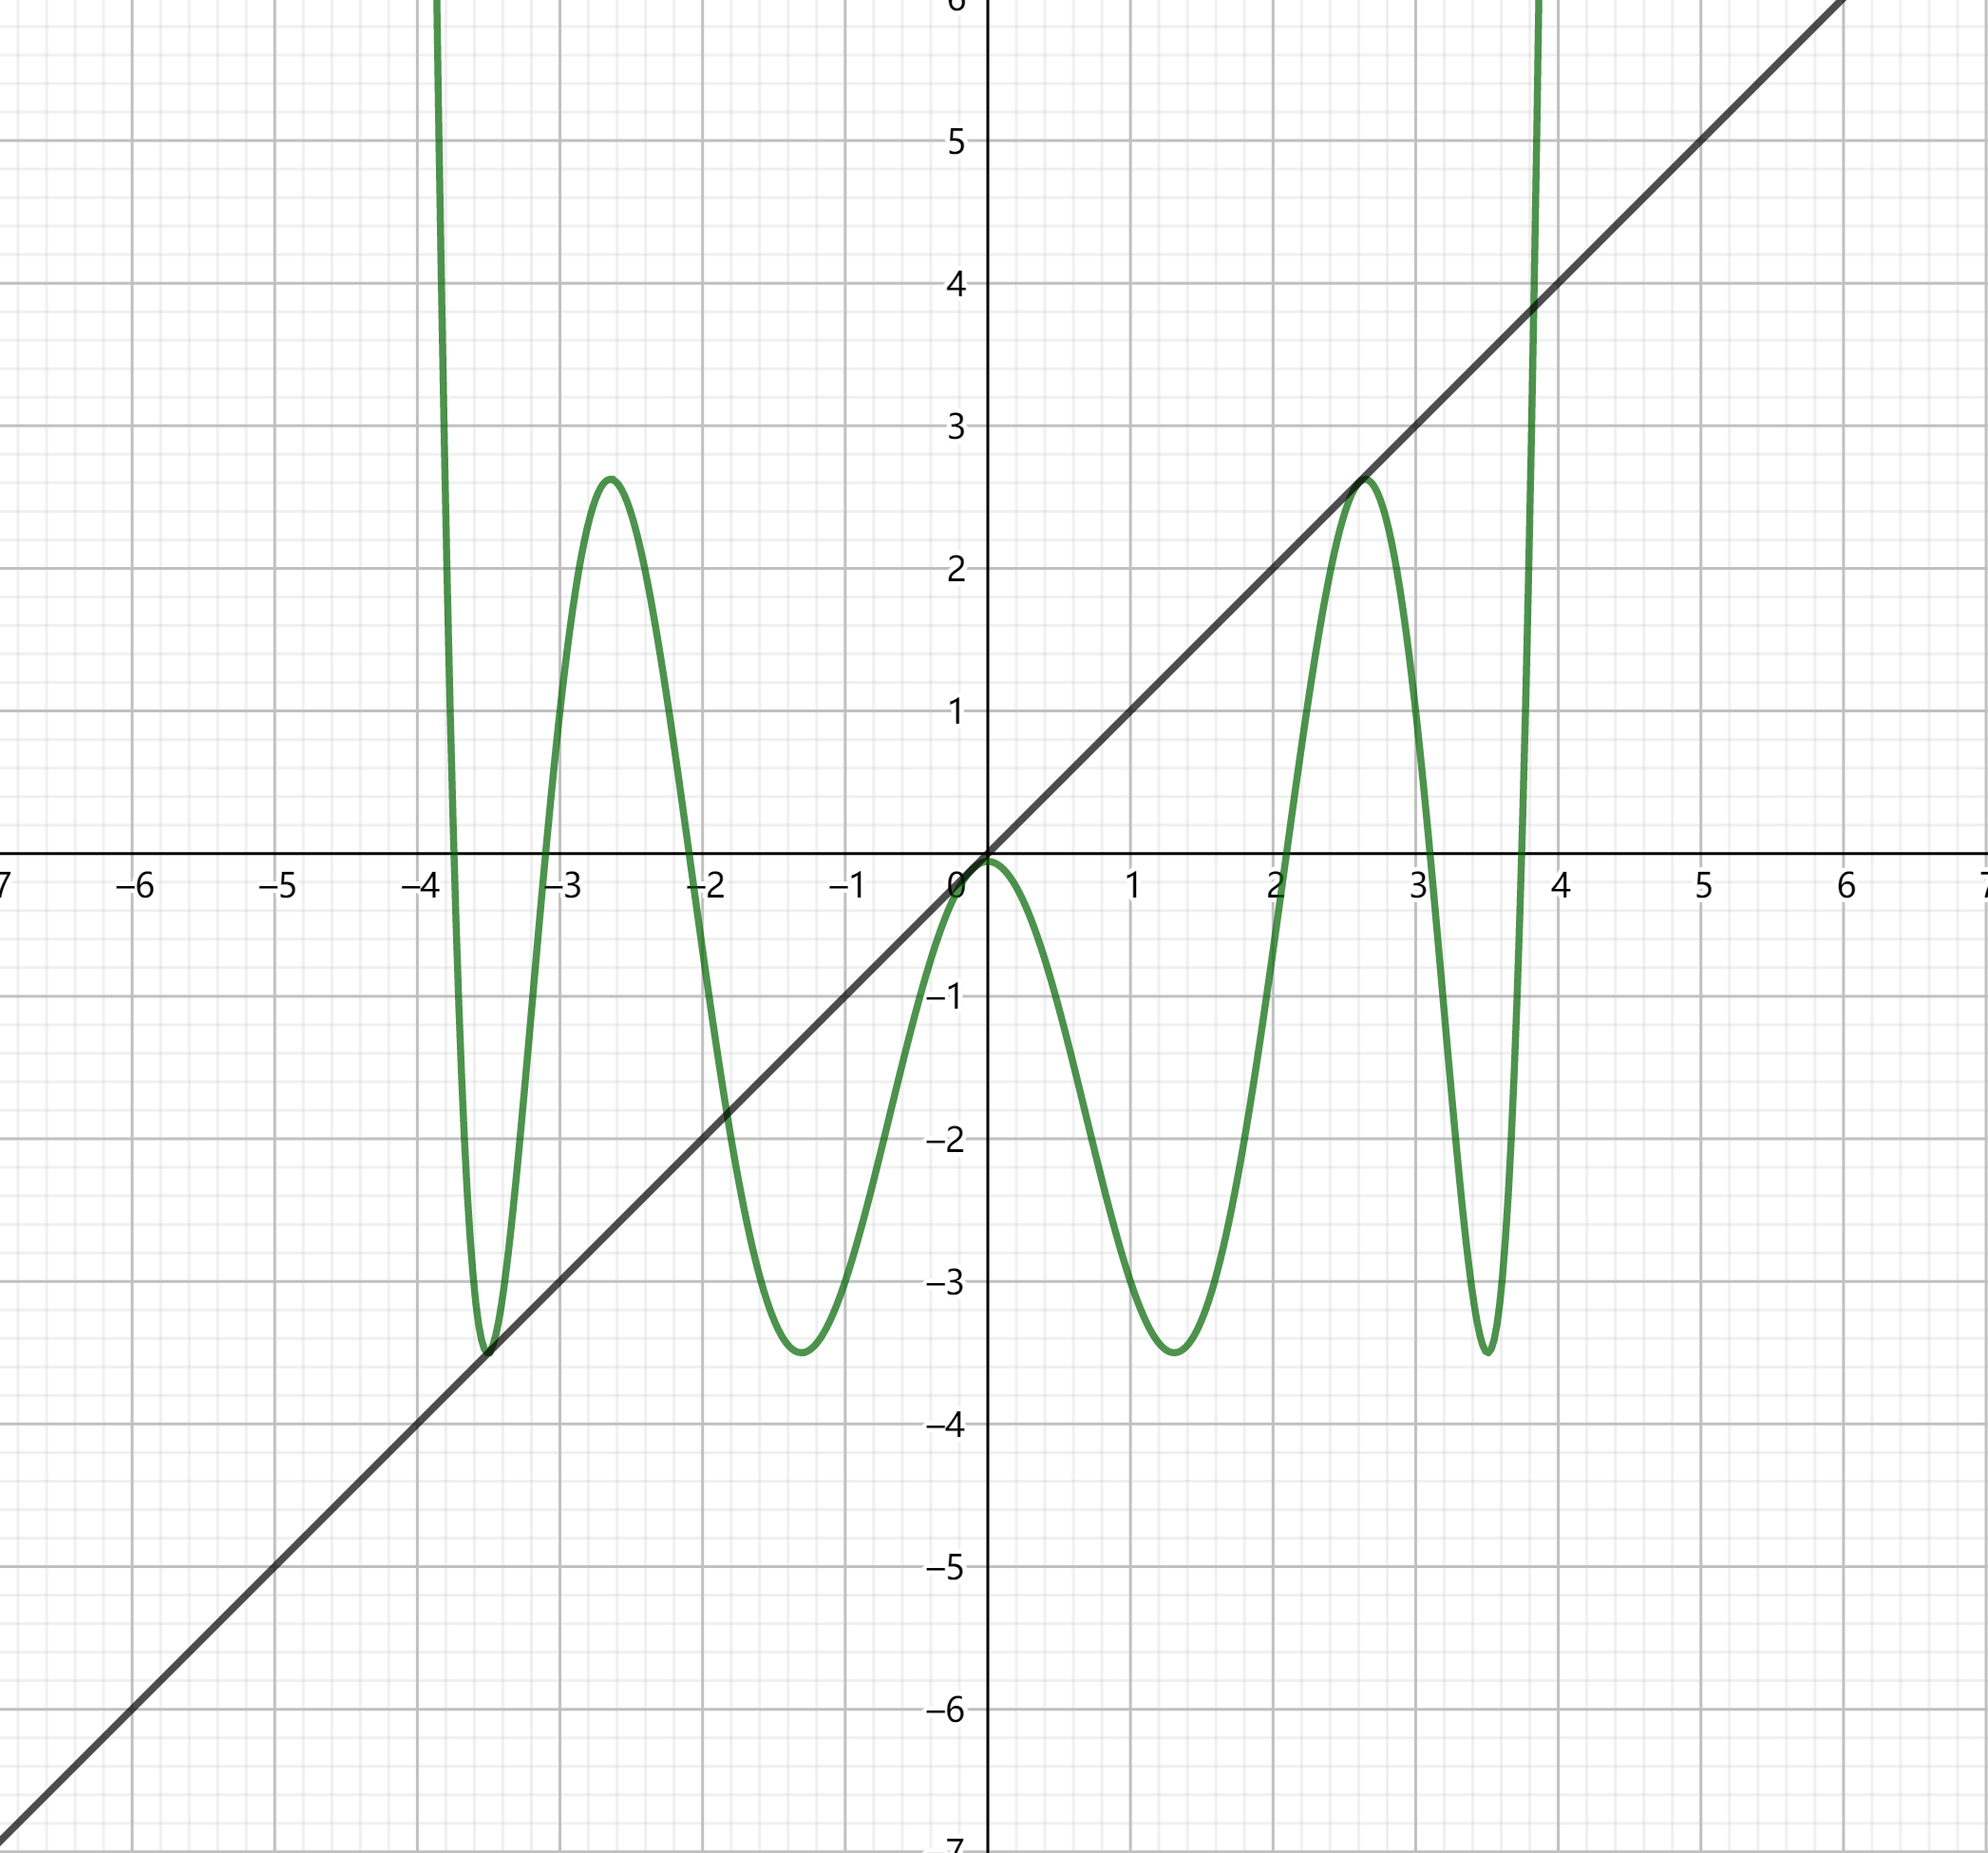
\includegraphics[scale=0.7]{图五}
    \caption[图五]{$c=-7$}\label{fig-图五}
    \end{figure}
%图六(无标题)
\begin{figure}[H]
    \centering
    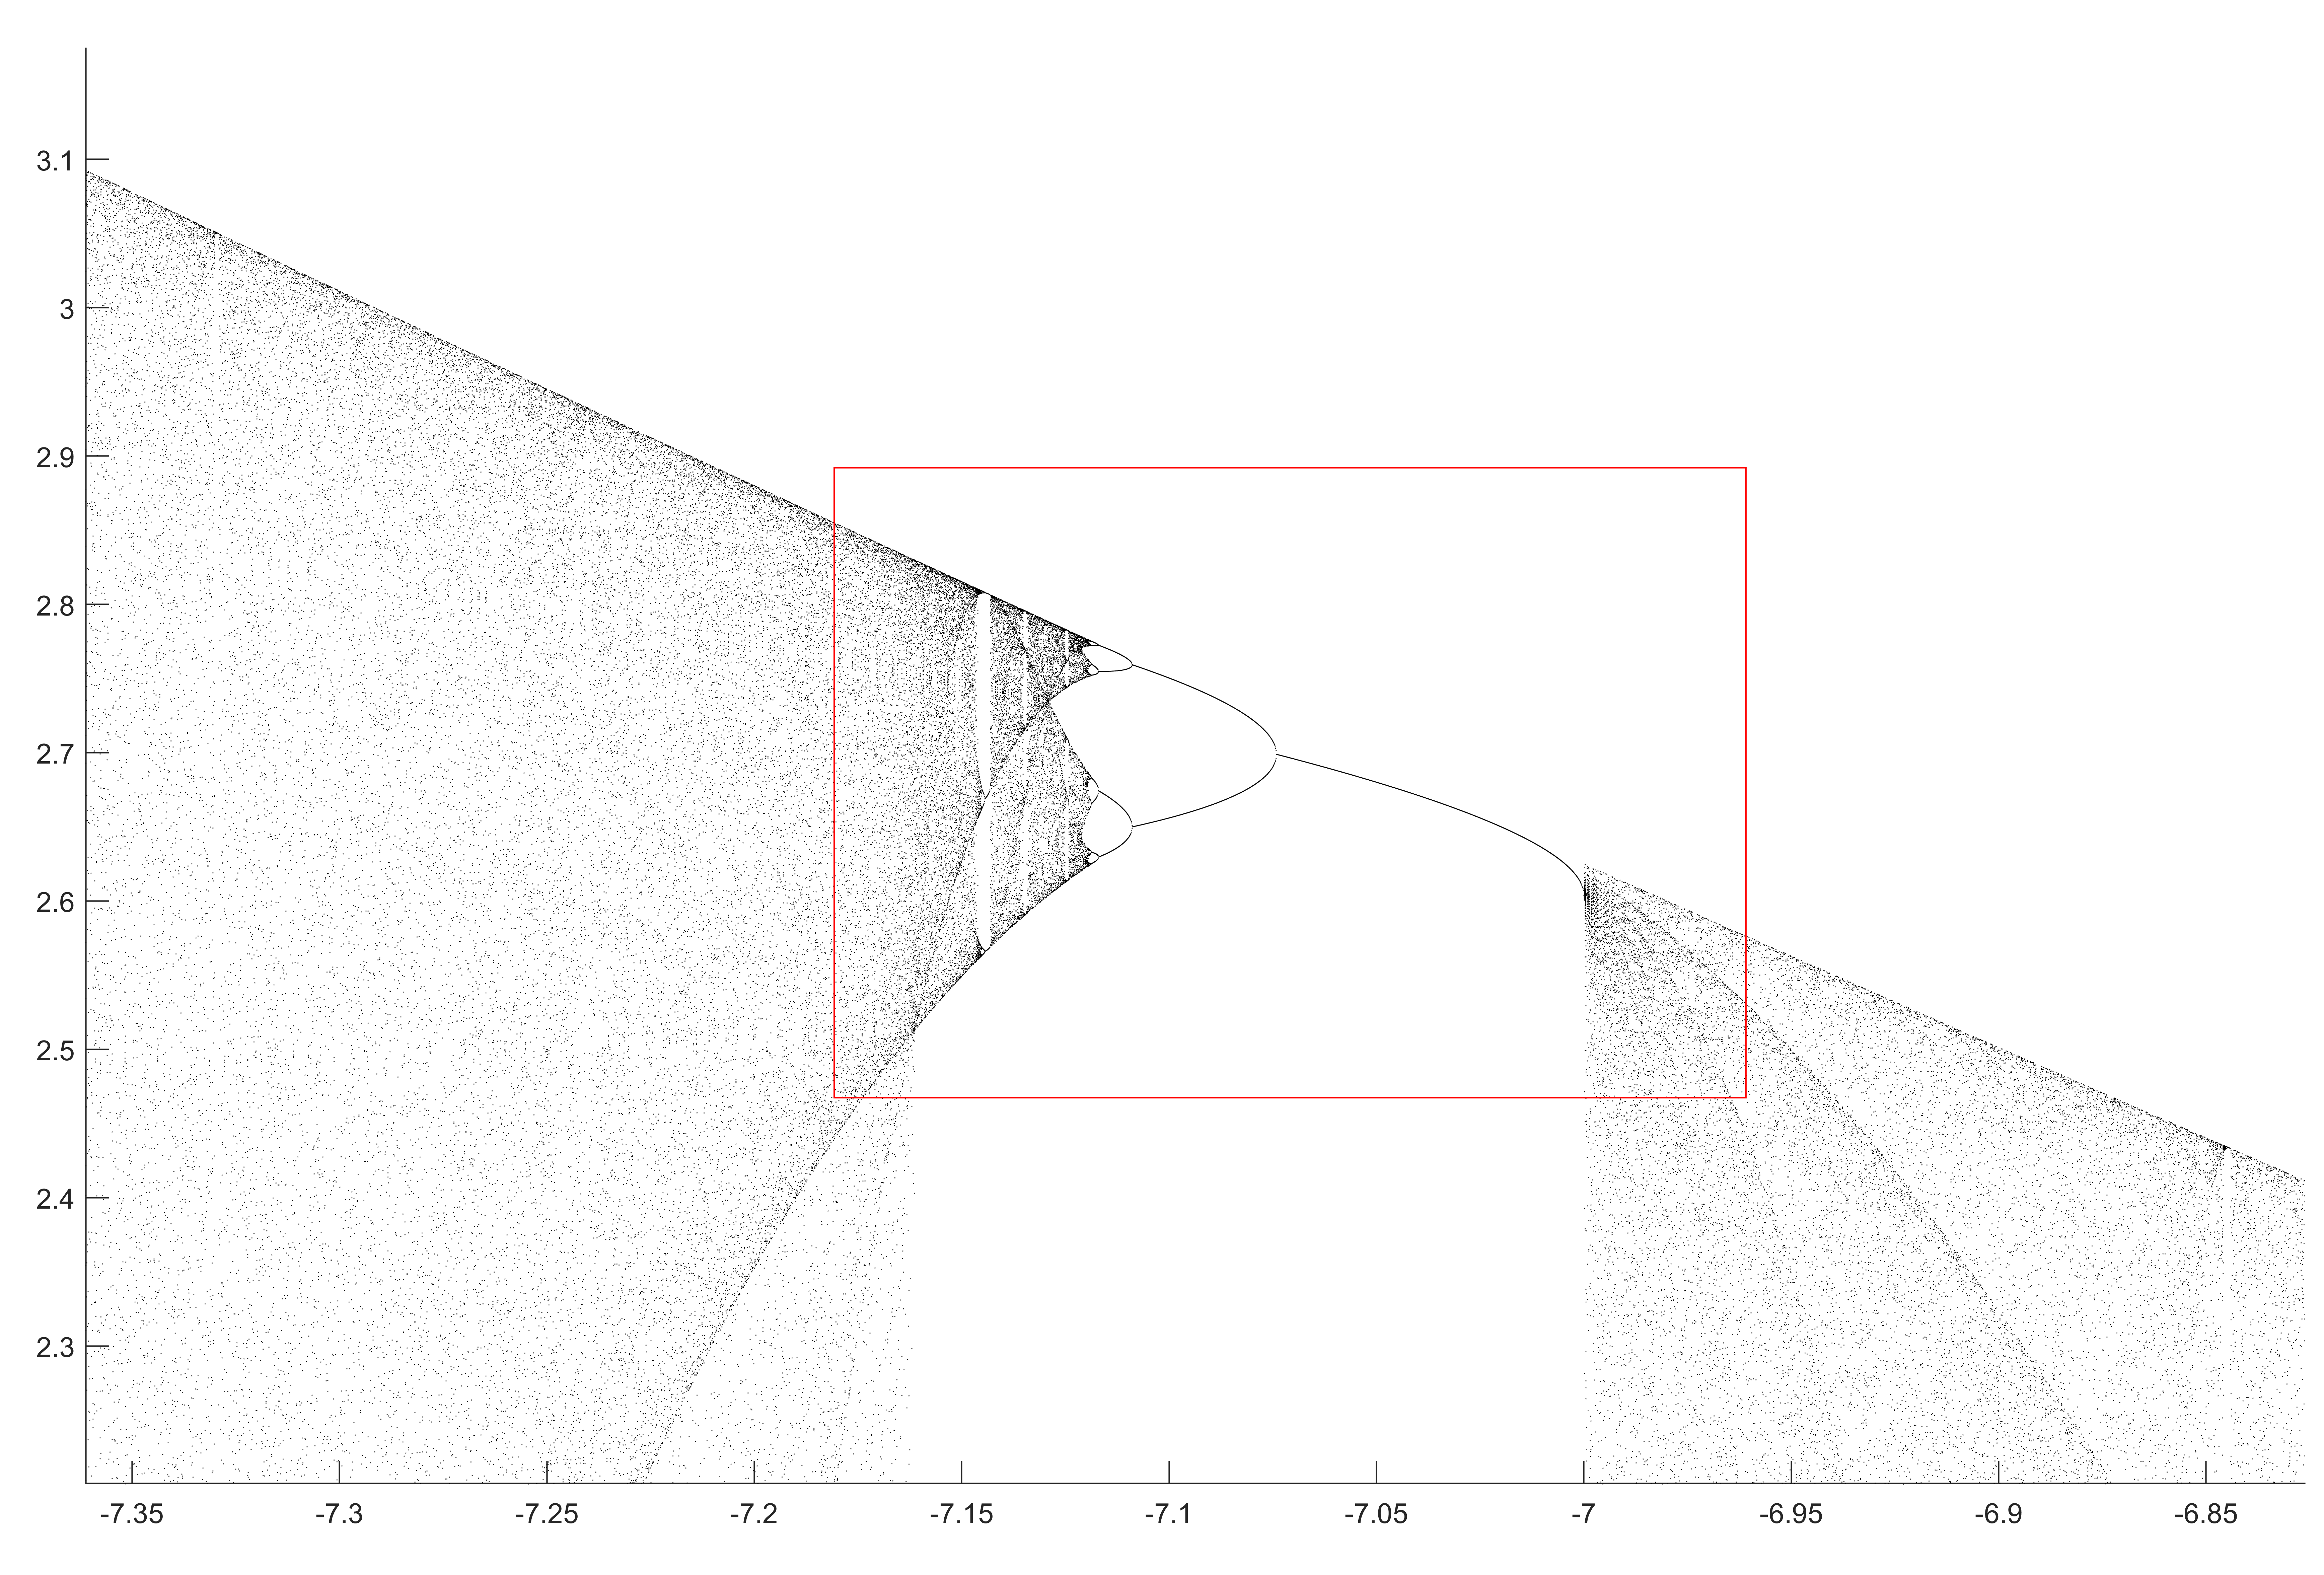
\includegraphics[scale=0.4]{图六}
    \caption[图六]{}\label{fig-图六}
    \end{figure}
同时,相切分岔还会产生混沌运动中的“窗口”.“窗口”内的分岔结构像是$c\in(-8,1)$的分岔图的缩微版本,如图6所示对应周期之比为该窗口对应的周期.

\begin{thm}对于$F:J\to J$,如果J中有一个周期为3的周期点,那么对于每个整数$n=1,2,3,\ldots $,存在有周期n的周期点,并且,有无穷多个J的子集,其中的元素甚至不会“渐进地具有周期性".\cite{d}\end{thm}

由此可知迭代数列$x_{n+1}=\frac{1}{2}x_{n}^2+\frac{1}{2}c$对于任意的正整数周期都有对应的周期点,同时也有无穷多个不具任何周期性的解.这种现象也被Li\&Yorke称为混沌.\cite{d}
%插入图七,标题为:总览
\begin{figure}[htb]
    \centering
    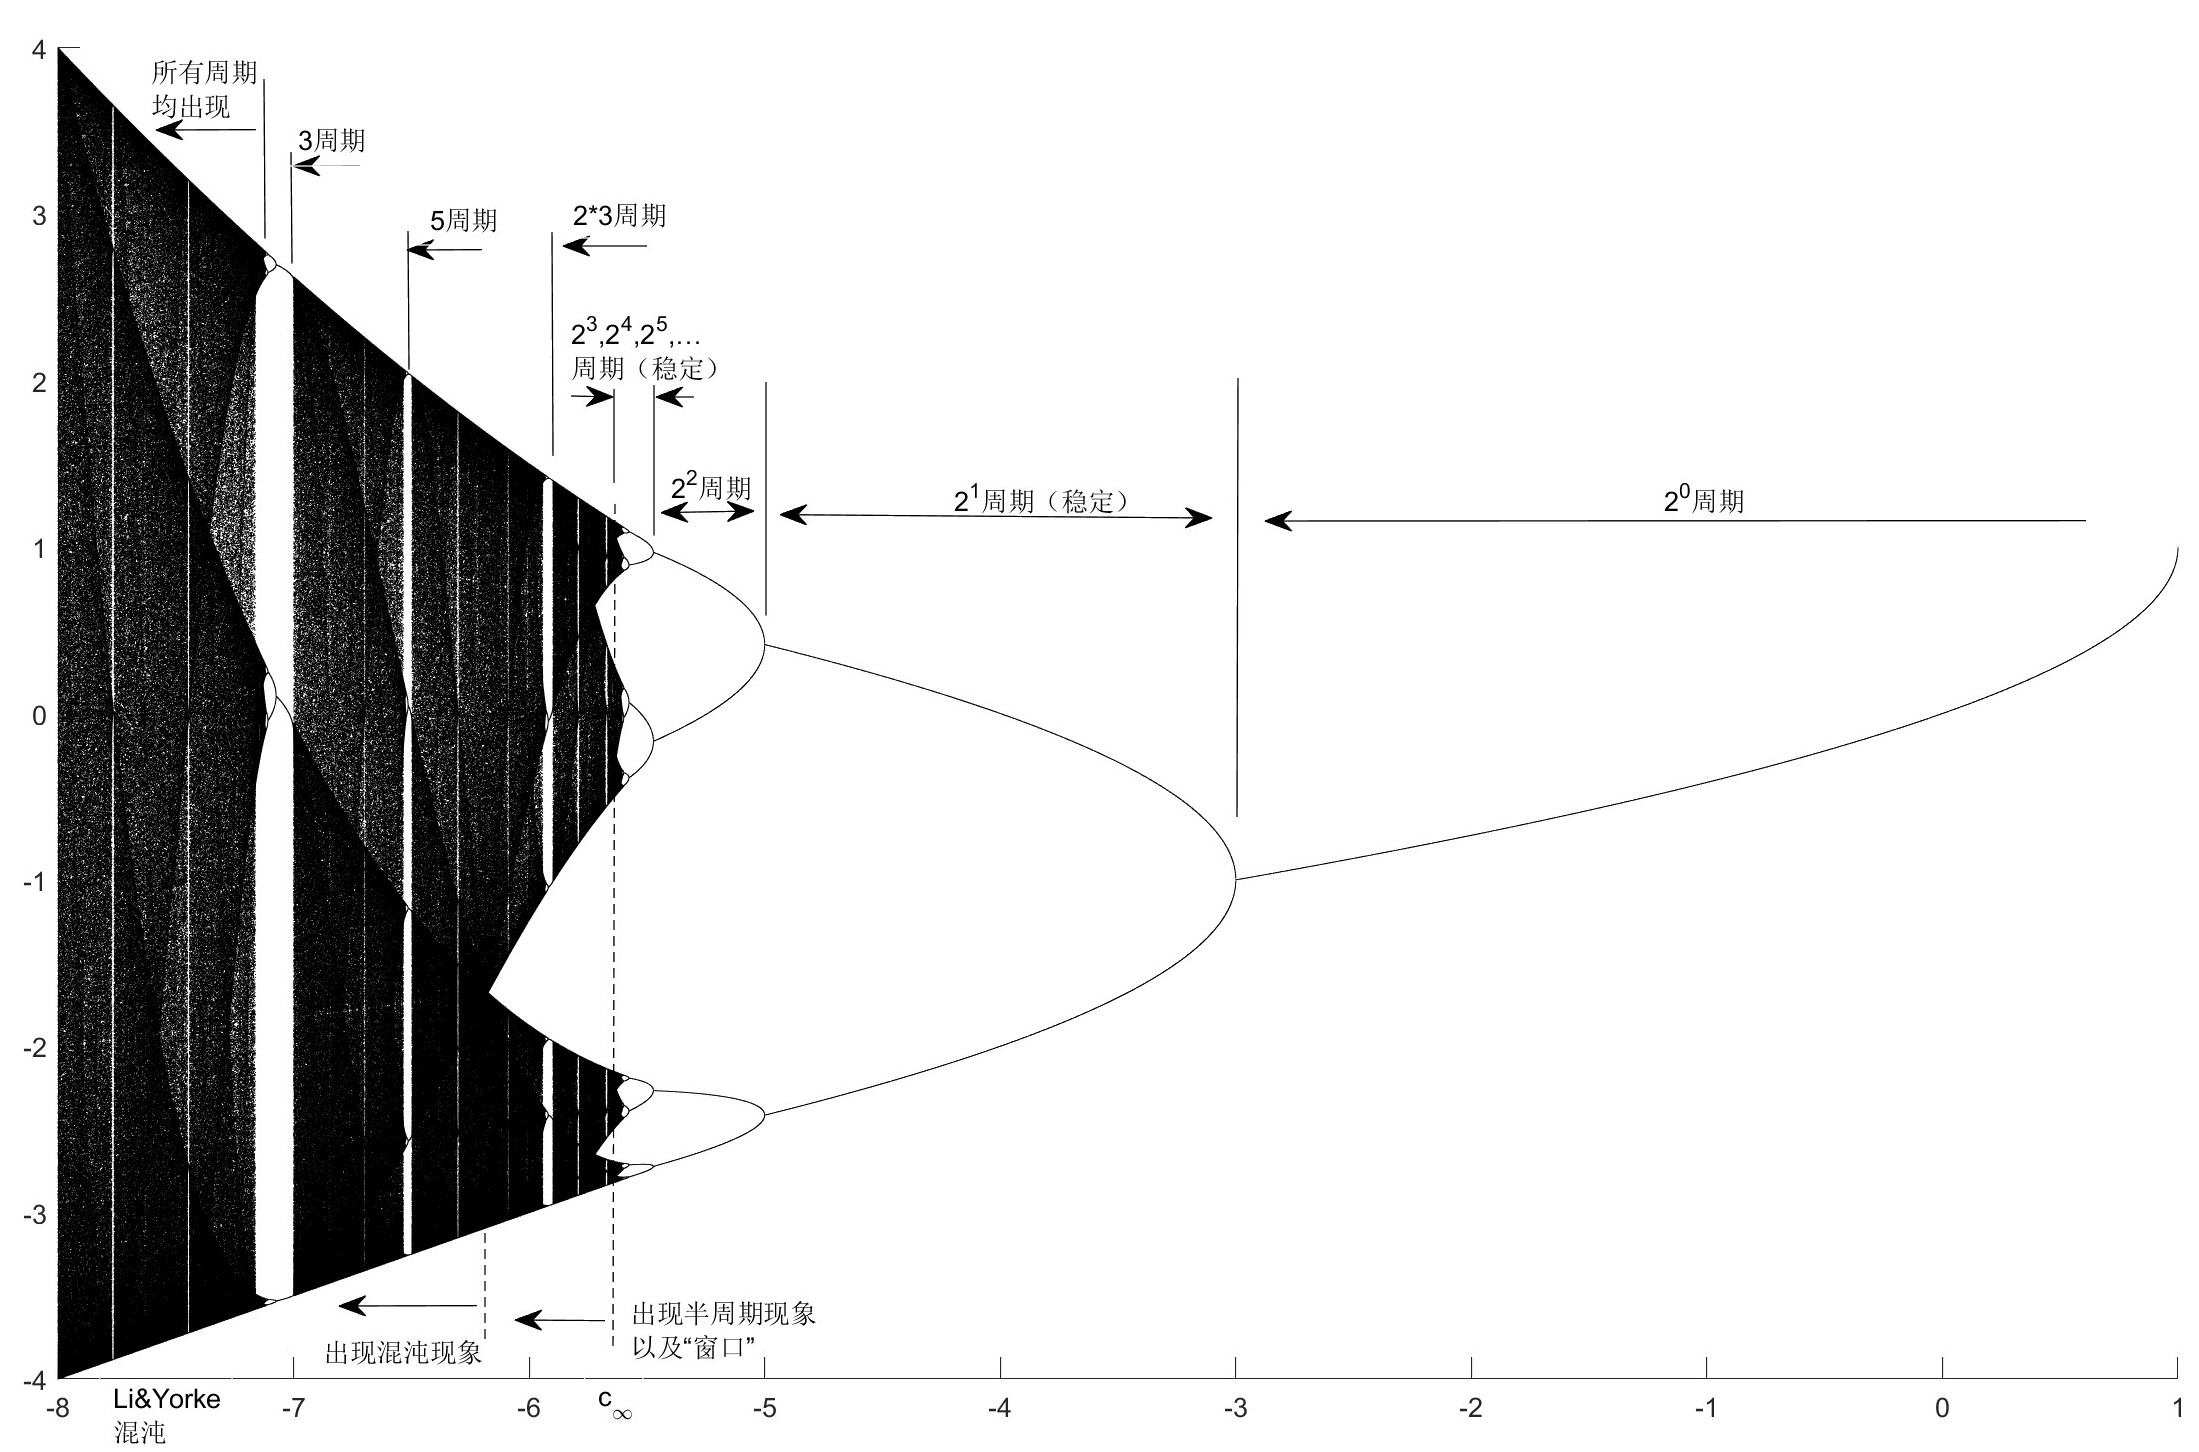
\includegraphics[scale=0.275]{图七}
    \caption[图七]{总览}\label{fig-图七}
    \end{figure}
\bibliography{math}
\end{document}

